\EXERCISE
پس از خراب‌کاری آقا محمود در جی‌جی‌کالا در روز افتتاحیه، آقا محمود اخراج شده و تصمیم گرفته‌است که در شرکت تپ‌چهل کار کند. بدین منظور برای استخدام مصاحبه‌ای برای آقا محمود تدارک دیده شده‌است. در این مصاحبه دایره‌ای در اختیار او قرار داده شده‌است که
$n$
$(n \geq 1)$
عدد حقیقی روی آن نوشته شده‌است که مجموع این اعداد برابر با
$1$
است. آقا محمود می‌تواند از یک عدد دل‌خواه شروع کرده و به ترتیب ساعت‌گرد اعداد را بخواند و
$n$
عدد خوانده شده را به ترتیب در
$1^3, 2^3, \cdots, n^3$
ضرب کند. از آقا محمود خواسته شده‌است که از جایی از دایره کار را شروع کند که نتیجه‌ی به‌دست آمده، بزرگ‌تر یا مساوی
$\frac{n^3}{4}$
باشد. آقا محمود که می‌ترسد مسئله‌ی داده شده برای سرِ کار گذاشتن او باشد، از شما خواسته‌است که اثبات کنید چنین عددی وجود دارد. مثلا در شکل زیر،
$n = 4$
است:
\begin{center}
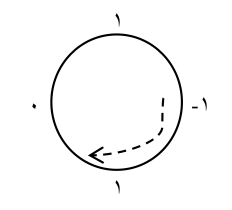
\includegraphics[height=3cm]{8.png}
\end{center}
اگر از عدد
$-1$
کار را آغاز کنیم مجموع برابر می‌شود با:
$$(-1) \times 1^3 + 1 \times 2^3 + 0 \times 3^3 + 1 \times 4^3 = 71$$